\documentclass[a4paper,11pt]{article}
\usepackage{xcolor}
\usepackage{geometry}
\usepackage{hyperref}
\hypersetup{
    colorlinks=false,
    linkcolor=blue,
    linkbordercolor=blue,
    pdfborderstyle={/S/U/W 1}
}
\usepackage{graphicx}
\usepackage{float}
\geometry{
a4paper,
total={170mm,257mm},
left=20mm,
top=20mm,
marginparsep=0mm,
}
\setlength\parindent{0pt} % get rid of the stupid indent

\title{DSD Theory Cheatsheet}
\author{Thomas Boxall\\ \texttt{up2108121@myport.ac.uk}}
\date{May 2023}

\usepackage{fancyhdr}
\pagestyle{fancy}
\fancyhead{} % clear all header fields
\renewcommand{\headrulewidth}{0pt} % no line in header area
\fancyfoot{} % clear all footer fields
\renewcommand{\footrulewidth}{0.4pt}
\fancyfoot[C]{\thepage} % page number in centre of the page
\fancyfoot[R]{\footnotesize Thomas Boxall\\ \texttt{up2108121@myport.ac.uk}} % right hand footer has author name on top line and author contact on bottom line
\fancyfoot[L]{\footnotesize DSD Theory Cheatsheet \\ May 2023} % left hand footer has title of document on top line and date on bottom line


\begin{document}

\maketitle
\thispagestyle{fancy}

\section{Data}
\textbf{Data} is facts and statistics collected together for reference or analysis.\\
\textbf{Information} is the result of processing data by adding context and meaning. We should carefully examine the context before drawing information from data.

\section{Database Management System}
The \textit{DataBase Management System} (DBMS) is the core of the database system. All communication to the database goes through DBMS. \\
DBMS controls users, access to data \& schema and provides an view of operations. DBMS removes risk of inconsistent data \& improves the ease which security can be controlled with.\\
Two different languages are used to interface with a database. \textit{Data Definition Language} (DDL) defines the structure of the database. \textit{Data Manipulation Language} (DML) is used to manipulate the data. 

\section{Entities \& where we keep them}
\textbf{Entity} a `thing' about which data is stored (often will be nouns). These should be singular, not plural.\\
\textbf{Attribute} a quality of an entity (eg id number, name, etc)\\
\textbf{Table} A 2D representation of entities. (AKA relation table or relation).\\
\textbf{Record} a row of data in a table. (AKA tuple or row).\\
\textbf{Relationship} is how two tables are related to each other, they are represented in relations. \\
When designing a database we have to think about the entities we will store, what data about them we need, and what form this data will take.

\subsection{Entity Relationship Diagrams}
\textbf{ERD} a diagram showing how entities \& attributes are related. They are built from business rules (\textit{statements that define how companies do things}). Entities are joined up using `Crows Foot Notation' (Figure \ref{fig:crow-foot-notation}).
\begin{figure}[ht]
    \centering
    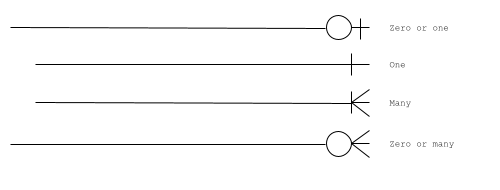
\includegraphics[width=0.9\textwidth]{../assets/relationship-links.png}
    \caption{Crow's foot notation}
    \label{fig:crow-foot-notation}
\end{figure}

\section{Keys}
\textbf{Primary Key} an attribute (or combination of attributes) which uniquely identifies a record. Every table must have one.\\
\textbf{Composite Key} a combination of attributes (each called simple keys) that act as a primary key in a table.\\
\textbf{Foreign Key} an attribute (or combination of attributes) which is a primary key in another table.\\
\textbf{Alternate Key} gives an alternate access path to data that is not via the primary key. This is \textit{bad} and if correctly normalised, this shouldn't exist. 

\section{Attributes}
\textbf{Constraint} a rule that protects your data or enforces certain behaviour.\\
All the different bits of data we store about an entity will all be different attributes. The data we store has to be GDPR compliant (must be: adequate, relevant and limited to what is necessary).
\subsection{Data Types}
\textit{see \href{https://thomasboxall.github.io/uni-notes/01-FIRST-YEAR/M30232-databaseSystemsDevelopment/M30232.pdf}{my notes} for more details on each data type.}\\
\textbf{Numerical} smallint, integer, bigint, decimal, real, double, serial, bigserial\\
\textbf{Alphanumeric} text, char, varchar\\
\textbf{Date \& time} timestamp without timezone, timestamp with timezone, date, time without timezone, time with timezone.

\section{Normalisation}
\textbf{Normalisation} the process of designing a database in a way that reduces data redundancy and makes the database more efficient.\\
\textbf{Data Redundancy} where there is repeated data, for example storing the full details of each boatyard with each employee.\\
There are many \textit{normal forms}, we are only concerned with 1st through 3rd.
\subsection{First Normal Form}
\begin{itemize}
    \item Each column should contain single (atomic) values (each column should not hold more than one value)
    \item Values stored in a column should be of the same domain (data type)
    \item All the columns in a table should have unique names
    \item The order in which the data is stored doesn't matter
\end{itemize}
Quite often when normalising to 1NF, you will find that a new entity gets created.

\subsection{Second Normal Form}
\begin{itemize}
    \item Be in 1NF
    \item Have no partial dependencies (where a part of a record can be identified by something other than the primary key)
\end{itemize}

\subsection{Third Normal Form}
\begin{itemize}
    \item Be in 2NF
    \item Have no transitive dependencies (where an attribute is dependent on an attribute which is not the primary key)
\end{itemize}

\section{Joins}
\begin{figure}[ht]
    \centering
    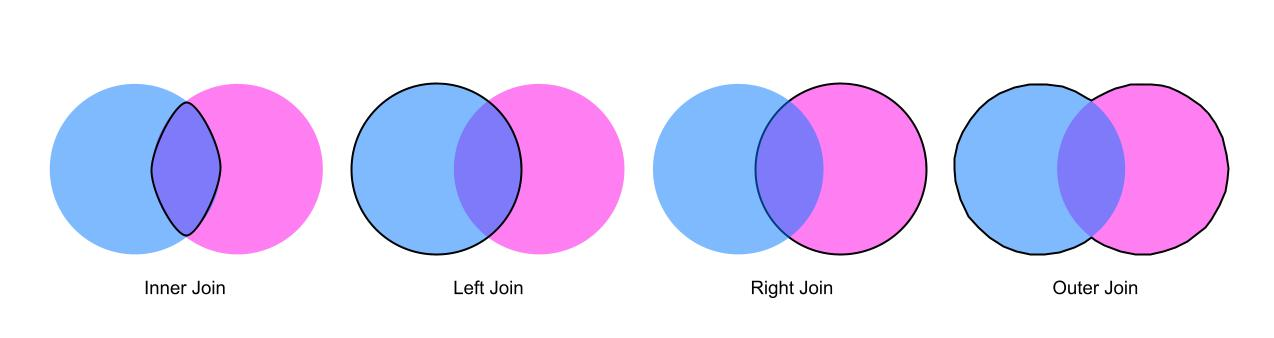
\includegraphics[width=0.9\textwidth]{../assets/joins.jpg}
    \caption{Joins}
    \label{fig:joins}  
\end{figure}
\textbf{Joins} allow us to join multiple tables together to get more data out of the database from a single query. Figure \ref*{fig:joins} shows the different types of joins.\\
\textbf{Cartesian Product} is the result of a bad join where the DBMS will return every record in one table is joined to every record in a second table. To avoid this, we tell the DBMS what attributes to match. \\
\textbf{Inner join} returns all the data where there is overlap in both tables. The overlap is decided base on the joining attribute.\\
\textbf{Left join} returns all the records in the left table with the entries of the right table where there is a match on the joining attribute.\\
\textbf{Right join} returns all the records in the right table with the entries of the left tables where there is a match on the joining attribute.\\
\textbf{Full outer join} returns everything from the two tables.\\
When joining two tables together, remember to use the correct type of join and to match the joining attribute (remember these may have different names in different tables). 

\section{Order Of Execution}
When executing a query, the DBMS will run statements in a different order to that which we enter them in.
\begin{enumerate}
    \item \verb|FROM| \& \verb|JOIN| (choose and join the tables to get base data)
    \item \verb|WHERE|, \verb|SUBQUERY|, \verb|INTERSECTION|, \verb|UNION|, \verb|EXCEPT| (filters the base data)
    \item \verb|GROUP BY| (aggregates the base data)
    \item \verb|HAVING| (filters the aggregated data)
    \item \verb|SELECT| (returns the final data, not displayed yet)
    \item \verb|ORDER BY| (sorts the final data)
    \item \verb|LIMIT| (limits the returned data to a row count)
    \item display data
\end{enumerate}

\section{Security}
To steal data, you just have to make a copy of it. The biggest security risk is those who have access to it.\\
\textbf{Superuser} is the top-level administrator in PostgreSQL. These accounts can do \textit{everything} so giving someone this role should be minimised as much as possible.
\subsection{Roles}
Before a user (role) can log into the DBMS, they have to have a role created and own a database with the same name as their username. Passwords must be set at the time of user creation, users should change passwords frequently. Once a user has been created, they have no permissions other than login. You have to grant permissions to users to perform actions.\\
\textbf{Views} can be used as a way of limiting user access to data. They allow pre-written queries to be executed which can only show \textit{some} data.
\subsection{Encryption}
By default (out of the box), encryption in PostgreSQL is disabled. It must be enabled before use.\\
A number of different hashing and data security options are available, including: PGP, md5, sha1, and sha255.\\
\textbf{Salt} can be added to data which is being encrypted to ensure every encrypted value is different, even if the values to be encrypted are the same. 


\end{document}